\documentclass[tikz,border=8pt]{standalone}
\usepackage{newtxtext,newtxmath}
\usetikzlibrary{arrows.meta,calc,positioning}

\definecolor{nnblue}{RGB}{223,242,250}
\definecolor{ariagold}{RGB}{255,246,214}
\definecolor{ariastroke}{RGB}{178,119,0}
\definecolor{softgray}{RGB}{245,245,245}

\begin{document}
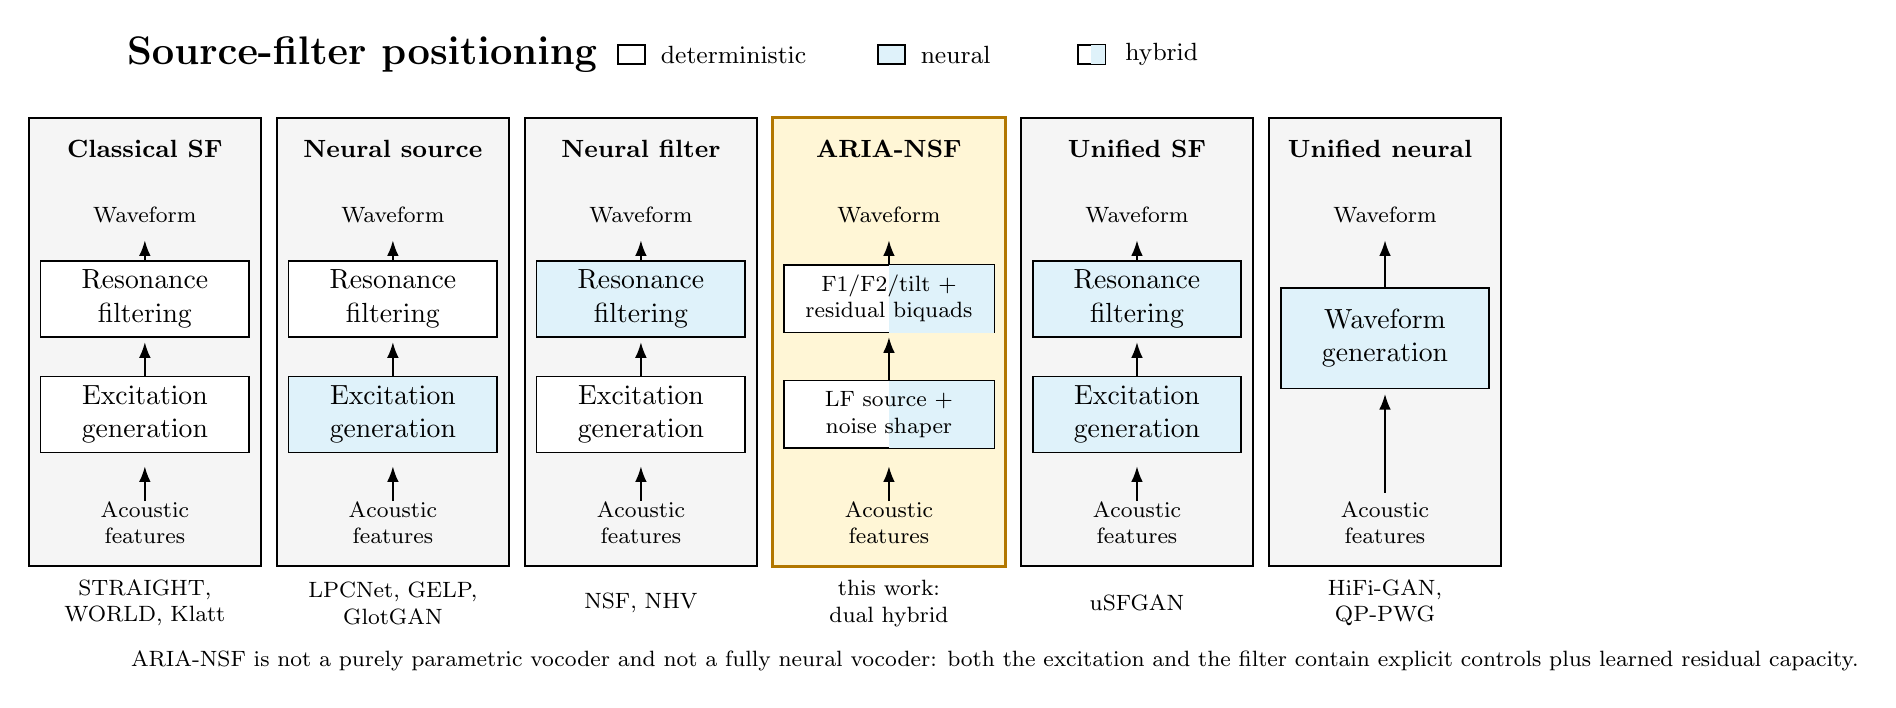
\begin{tikzpicture}[
  font=\rmfamily,
  >={Latex[length=2.0mm,width=1.35mm]},
  arrow/.style={-Latex, line width=0.58pt, shorten >=1.7pt},
  box/.style={draw, line width=0.65pt, minimum width=2.65cm, minimum height=0.86cm, align=center, fill=white},
  nnbox/.style={box, fill=nnblue},
  genbox/.style={draw, line width=0.65pt, minimum width=2.65cm, minimum height=1.28cm, align=center, fill=nnblue},
  label/.style={font=\rmfamily\small, align=center},
  tiny/.style={font=\rmfamily\footnotesize, align=center},
  model/.style={draw, line width=0.75pt, minimum width=2.95cm, minimum height=5.70cm, inner sep=0pt, fill=softgray},
  ariamodel/.style={model, draw=ariastroke, line width=1.05pt, fill=ariagold}
]

\node[anchor=west, font=\rmfamily\Large\bfseries] at (-0.35,3.65) {Source-filter positioning};

% Legend
\node[box, minimum width=0.34cm, minimum height=0.24cm, anchor=west] at (6.0,3.65) {};
\node[anchor=west, font=\rmfamily\small] at (6.43,3.65) {deterministic};
\node[nnbox, minimum width=0.34cm, minimum height=0.24cm, anchor=west] at (9.30,3.65) {};
\node[anchor=west, font=\rmfamily\small] at (9.73,3.65) {neural};
\draw[fill=white, draw, line width=0.65pt] (11.85,3.53) rectangle (12.19,3.77);
\draw[fill=nnblue, draw=none] (12.02,3.53) rectangle (12.19,3.77);
\node[anchor=west, font=\rmfamily\small] at (12.33,3.65) {hybrid};

\foreach \x/\name in {
0/Classical SF,
3.15/Neural source,
6.30/Neural filter,
9.45/ARIA-NSF,
12.60/Unified SF,
15.75/Unified neural
}{
  \ifdim\x pt=9.45pt
    \node[ariamodel] (m\x) at (\x,0) {};
  \else
    \node[model] (m\x) at (\x,0) {};
  \fi
  \node[label, font=\rmfamily\bfseries\small] at (\x,2.45) {\name};
}

% Reusable vertical coordinates
\foreach \x in {0,3.15,6.30,9.45,12.60} {
  \node[tiny] at (\x,-2.30) {Acoustic\\features};
  \draw[arrow] (\x,-2.02) -- (\x,-1.52);
}

% Classical
\node[box] (e0) at (0,-0.92) {Excitation\\generation};
\node[box] (f0) at (0,0.55) {Resonance\\filtering};
\node[tiny] at (0,1.62) {Waveform};
\draw[arrow] (e0) -- (f0);
\draw[arrow] (f0.north) -- (0,1.35);
\node[tiny] at (0,-3.32) {STRAIGHT,\\WORLD, Klatt};

% Neural source + parametric filtering
\node[nnbox] (e1) at (3.15,-0.92) {Excitation\\generation};
\node[box] (f1) at (3.15,0.55) {Resonance\\filtering};
\node[tiny] at (3.15,1.62) {Waveform};
\draw[arrow] (e1) -- (f1);
\draw[arrow] (f1.north) -- (3.15,1.35);
\node[tiny] at (3.15,-3.32) {LPCNet, GELP,\\GlotGAN};

% Parametric source + neural filtering
\node[box] (e2) at (6.30,-0.92) {Excitation\\generation};
\node[nnbox] (f2) at (6.30,0.55) {Resonance\\filtering};
\node[tiny] at (6.30,1.62) {Waveform};
\draw[arrow] (e2) -- (f2);
\draw[arrow] (f2.north) -- (6.30,1.35);
\node[tiny] at (6.30,-3.32) {NSF, NHV};

% ARIA hybrid source and hybrid filter
\draw[fill=white, draw, line width=0.65pt] (8.12,-1.35) rectangle (10.78,-0.49);
\draw[fill=nnblue, draw=none] (9.45,-1.35) rectangle (10.78,-0.49);
\node[tiny] (e3) at (9.45,-0.92) {LF source +\\noise shaper};
\draw[fill=white, draw, line width=0.65pt] (8.12,0.12) rectangle (10.78,0.98);
\draw[fill=nnblue, draw=none] (9.45,0.12) rectangle (10.78,0.98);
\node[tiny] (f3) at (9.45,0.55) {F1/F2/tilt +\\residual biquads};
\node[tiny] at (9.45,1.62) {Waveform};
\draw[arrow] (9.45,-0.49) -- (9.45,0.12);
\draw[arrow] (9.45,0.98) -- (9.45,1.35);
\node[tiny] at (9.45,-3.32) {this work:\\dual hybrid};

% Unified source-filter
\node[nnbox] (e4) at (12.60,-0.92) {Excitation\\generation};
\node[nnbox] (f4) at (12.60,0.55) {Resonance\\filtering};
\node[tiny] at (12.60,1.62) {Waveform};
\draw[arrow] (e4) -- (f4);
\draw[arrow] (f4.north) -- (12.60,1.35);
\node[tiny] at (12.60,-3.32) {uSFGAN};

% Unified neural generation
\node[tiny] (ac5) at (15.75,-2.30) {Acoustic\\features};
\node[genbox] (g5) at (15.75,0.05) {Waveform\\generation};
\node[tiny] at (15.75,1.62) {Waveform};
\draw[arrow] (ac5.north) -- (g5.south);
\draw[arrow] (g5.north) -- (15.75,1.35);
\node[tiny] at (15.75,-3.32) {HiFi-GAN,\\QP-PWG};

\node[anchor=west, font=\rmfamily\footnotesize, align=left] at (-0.30,-4.05)
{ARIA-NSF is not a purely parametric vocoder and not a fully neural vocoder: both the excitation and the filter contain explicit controls plus learned residual capacity.};

\end{tikzpicture}
\end{document}
